\documentclass[notes,color]{sepslide0}
\usepackage{graphicx}
\usepackage[overheads]{mysepslides}
\usepackage{tech,graphicx,url,tikz,scalalistings}

\title{Semaphores} 
\author{Gavin Lowe}

\everymath{\color{violet}}
\def\scalacolour{\color{violet}}
\def\codecolour{\scalashape}

\begin{document}

\begin{slide}
  
  \Title

Reading: Andrews Chapter 4.
\end{slide}

%%%%%%%%%%%%%%%%%%%%%%%%%%%%%%%%%%%%%%%%%%%%%%%%%%%%%%%


\begin{slide}
\heading{Semaphores}

A semaphore is an important synchronisation tool.  The idea (and name) is
inspired by railway signalling, where a flag is raised to indicate that track
ahead can be entered, or lowered to indicate that the track ahead is occupied.
A train arriving at the section of track waits until the flag is up, enters
the section, and the flag is lowered again.  When the train leaves the section
of track, the flag is raised. 

A semaphore 
%% has a boolean variable, that indicates whether the flag is down.  It
has two operations:
%
\begin{description}
\item[{down}]
Wait until the flag is in the up position, and then put the flag down and
procced;

\item[{up}]
Put the flag up, to allow another process to proceed.
\end{description}

\SCALA{down} and \SCALA{up} are sometimes called \SCALA{P} and \SCALA{V},
{\codecolour\sf wait} and \SCALA{signal}, or \SCALA{acquire} and
\SCALA{release}. 
\end{slide}

%%%%%

\begin{slide}
\heading{Semaphores in Scala}

A semaphore can be implemented as a monitor, as below.
%
\begin{scala}
/** A binary semaphore.
  * @param isUp is the semaphore initially in the "up" state? */
class Semaphore(private var isUp: Boolean){
  def down = synchronized{
    while(!isUp) wait()
    isUp = false
  }

  def up = synchronized{
    require(!isUp); isUp = true; notify()
  }
}
\end{scala}
% Note that |up| has no effect if the semaphore is already up. 
\end{slide}

%%%%%

\begin{slide}
\heading{Implementing semaphores}

Note that the |up| operation requires that the semaphore is not already up.
My experience is that trying to put the semaphore up when it is already up is
nearly always an error: a signal gets lost.

However, other implementations of semaphores allow such an |up|, but are such
that the operation has no effect. 

In fact, many operating system kernels provide implementations of semaphores.  

Semaphores can then be used to implement monitors within a programming
language. 

%% \bigskip

%% \heading{Semaphores in SCO}

%% The factory method |BooleanSemaphore(available)| creates a new semaphore.
%% (The method has various optional arguments, not included on the previous
%% slide.) 


\end{slide}

%%%%%

\begin{slide}
\heading{Using a semaphore for mutual exclusion}

One use of semaphores is to provide mutual exclusion.  

Such a semaphore is created with
\begin{scala}
  val mutex = new Semaphore(true)
\end{scala}
or
\begin{scala}
  val mutex = new MutexSemaphore
\end{scala}
%
using the definition
%
\begin{scala}
class MutexSemaphore extends Semaphore(true)
\end{scala}
\end{slide}

%%%%%

\begin{slide}
\heading{Using a semaphore for mutual exclusion}

A thread entering the critical region executes
\begin{scala}
  mutex.down
\end{scala}
%
This blocks if the semaphore is already down, i.e.~if another thread is in the
critical region.  In the initial state, the operation will not block. 

A thread leaving the critical region executes
\begin{scala}
  mutex.up
\end{scala}
%
This unblocks a waiting thread (if there is one).
\end{slide}

%%%%%

\begin{slide}
\heading{Using a semaphore for mutual exclusion}

This version of the counter protects \SCALA{x} using a semaphore.
%
\begin{scala}
object Counter{
  private var x = 0
  
  private var mutex = new MutexSemaphore
    
  def inc = { mutex.down; x = x+1; mutex.up }

  def dec = { mutex.down; x = x-1; mutex.up }

  def getX = { mutex.down; val result = x; mutex.up; result }
}
\end{scala}
%
% Note that this method can be used to provide mutual exclusion on arbitrary
% objects (like a monitor).
\end{slide}

%%%%%

\begin{slide}
\heading{Misusing semaphores}

What is wrong with the following code, where semaphore \SCALA{sem1} is used to
protect resource \SCALA{res1}, and semaphore \SCALA{sem2} is used to protect
resource \SCALA{res2}?
%
\begin{scala}
val sem1 = MutexSemaphore(); val sem2 = MutexSemaphore()

def p = proc{
  sem1.down; ...; sem2.down; ... ; sem2.up; ...; sem1.up
}

def q = proc{
  sem2.down; ...; sem1.down; ... ; sem1.up; ...; sem2.up
}

run(p || q)
\end{scala}
\end{slide}
 % introduction, use for mutex

\begin{slide}
\heading{Mutual exclusion using semaphores}

A semaphore that is used to enforce mutual exclusion is initially up.  A
process that enters the critical region does a \SCALA{down}, to block other
processes from entering.  When it leaves the critical region it does an
\SCALA{up}, to allow other processes to proceed.
\end{slide}

%%%%%


\begin{slide}
\heading{Signalling using semaphores}

By contrast a \emph{signalling semaphore} is initially down.  A process can
send a signal by performing an \SCALA{up}.  A process waits for a signal by
performing a \SCALA{down}.
\begin{scala}
private val signal = new Semaphore(false)
def signaller = proc{ ...; signal.up; ... }
def waiter = proc{ ...; signal.down; ... }
\end{scala}  
The \SCALA{waiter} cannot proceed before the signal is sent (but the
\SCALA{signaller} can proceed before the signal is received).

Note that the signal is received by only one other process.  Note also that if
the |signaller| performs the signal before the |waiter| is ready, the signal
is not lost.
\end{slide}

%%%%%

\begin{slide}
\heading{Signalling using semaphores}

Alternatively, the signalling semaphore can be created using
\begin{scala}
private val signal = new SignallingSemaphore
\end{scala}
via the definition
\begin{scala}
class SignallingSemaphore extends Semaphore(false)
\end{scala}
\end{slide}

%%%%%

\begin{slide}
\heading{Synchronising using semaphores}

Two processes can synchronise using a pair of signalling semaphores: each
signals to the other when it reaches the synchronisation point; neither
proceeds until it has received the signal from the other.
\begin{scala}
val signal1 = new SignallingSemaphore
val signal2 = new SignallingSemaphore
def p1 = proc{ ...; signal1.up; signal2.down; ... }
def p2 = proc{ ...; signal2.up; signal1.down; ... }
\end{scala}
\end{slide}

%%%%%

\begin{slide}
\heading{Synchronising using semaphores}

The code on the previous slide works fine if the threads use the semaphores to
synchronise just once.  However, it can go wrong if the threads use the same
semaphores to synchronise multiple times. 
%
\begin{scala}
def p1 = proc{ for(i <- 1 to 2){ ...; signal1.up; signal2.down; ... } }
def p2 = proc{ for(i <- 1 to 2){ ...; signal2.up; signal1.down; ... } }
\end{scala}
%
%% Consider an execution of the above where each thread should executes the loop
%% precisely twice.
The following sequence of events is possible, where the
subscripts represent the iteration number.
\[
\begin{align}
\sm{signal1.up}_1,\; \sm{signal2.up}_1,\; \sm{signal2.down}_1,\;
   \sm{signal1.up}_2
\end{align}
\]
Thread~|p2| is suspended after performing its first signal, so that |p1|
performs its second signal \emph{before} |p2| consumes the first signal. 
With our implementation of semaphores, the precondition of |up| is not
satisfied, and an exception is thrown. 
\end{slide}

%%%%%

\begin{slide}
\heading{Synchronising using semaphores}

If we had allowed an |up| when the semaphore is already up (and made it a
no-op), the execution would have continued something like:
\[
\begin{align}
\sm{signal1.up}_1,\; \sm{signal2.up}_1,\; \sm{signal2.down}_1,\;
   \sm{signal1.up}_2, \\
\sm{signal1.down}_1,\; \sm{signal2.up}_2,\; \sm{signal2.down}_2
\end{align}
\]
Here the second signal by |p1| is lost.  Subsequently, |p1| terminates, but
|p2| is stuck waiting for a second signal.
\end{slide}

%%%%%

\begin{slide}
\heading{Synchronising using semaphores}

A solution is to reverse the order of events in one of the threads.
\begin{scala}
def p1 = proc{ for(...){ ...; signal1.up; signal2.down; ... } }
def p2 = proc{ for(...){ ...; signal1.down; signal2.up; ... } }
\end{scala}
%
We can reason as follows (recall the ``happens before'' relation $\prec$).
\[
\begin{array}{rcl@{\qquad}l}
\sm{signal1.up}_1 & \prec & \sm{signal1.down}_1 & 
  \mbox{(signal on {\scalashape signal1})} \\
 & \prec & \sm{signal2.up}_1 & \mbox{(program order for \SCALA{p2})} \\
 & \prec & \sm{signal2.down}_1 & \mbox{(signal on {\scalashape signal2})} \\
 & \prec & \sm{signal1.up}_2 & \mbox{(program order for \SCALA{p1})} \\
 & \prec & \ldots
\end{array}
\]
In particular, the events happen in the expected order, and neither thread
completes the synchronisation on the $n$th iteration before the other thread
has signalled on that iteration.
%
The precondition of |up| is satisfied since $\sm{signal1.down}_n \prec
\sm{signal1.up}_{n+1}$, for each~$n$, and similarly for |signal2|.
\end{slide}

%%%%%

\begin{slide}
\heading{Example: a partial queue using semaphores}

We will implement a partial queue using semaphores.  

If a |dequeue| finds that the queue is empty, it will wait for a signal on a
signalling semaphore |dequeueWait|.  When a subsequent |enqueue| signals on
this semaphore, it will indicate that the queue is now non-empty (in fact,
that the queue contains precisely one element), and the dequeue can proceed.

In addition, we have to protect the shared variables from race conditions.  We
will use a |MutexSemaphore| for this. 

When an |enqueue| finishes, it will either signal on |dequeueWait| to a
waiting |dequeue| if there is one (and leave the mutex down), or lift the
mutex.  We record the number of waiting |dequeues| to support this.
\end{slide}

%%%%%

\begin{slide}
\heading{Example: a partial queue using semaphores}

\begin{scala}
class SemaphorePartialQueue[T] extends PartialQueue[T]{
  /** The queue itself. */
  private val queue = new scala.collection.mutable.Queue[T]

  /** Number of waiting dequeues. */
  private var waitingDequeues = 0

  /** Semaphore to provide mutual exclusion. */
  private val mutex = new MutexSemaphore

  /** Semaphore on which a dequeue waits until the queue is non-empty. */
  private val dequeueWait = new SignallingSemaphore

  // Invariant: if waitingDequeues > 0 and mutex is up, then the queue is empty.
  ...
}
\end{scala}
\end{slide}

%%%%%

\begin{slide}
\heading{Example: a partial queue using semaphores}

\begin{scala}
  def enqueue(x: T) = {
    mutex.down
    queue.enqueue(x)
    if(waitingDequeues > 0) dequeueWait.up // pass the baton to a dequeue at (1)
    else mutex.up
  }

  def dequeue: T = {
    mutex.down
    if(queue.isEmpty){  // have to wait
      waitingDequeues += 1; mutex.up
      dequeueWait.down                         // wait for signal (1)
      assert(queue.length == 1)
      waitingDequeues -= 1
    }
    val result = queue.dequeue; mutex.up; result
  }
\end{scala}
\end{slide}

%%%%%

\begin{slide}
\heading{Passing the baton}

The technique used by |enqueue| is known as \emph{passing the baton}.  It
decides what sort of operation should run next ---either a waiting dequeue or
a new operation--- and ``passes it the baton'' by lifting the appropriate
semaphore. 

Note that when a thread passes the baton to a thread waiting on a signalling
semaphore, it leaves the mutex semaphore down: the latter takes over the
rights implied by possession of the mutex.  

By contrast, the waiting thread should lift the mutex before waiting,
otherwise the system will deadlock.

The technique of passing the baton is quite generally applicable.  Often the
current thread is in the best position to decide which thread can run next.
\end{slide}

%%%%%

\begin{slide}
\heading{Barrier synchronisation}

Recall that a barrier synchronisation can be used to synchronise $n>1$
processes.  Each process in turn calls \SCALA{sync} on the barrier.  Once all
$n$ processes have called \SCALA{sync}, the processes can continue.
%% \end{slide}

%% %%%%%

%% \begin{slide}
%% \heading{Barrier synchronisation}

We define a class
\begin{scala}
class Barrier(n: Int){ def sync = { ... } }
\end{scala}%
%
to implement barrier synchronisation.  

We keep track of the number of threads currently waiting in a variable
\SCALA{waiting}.  We protect this using a mutex semaphore. 

We use a signalling semaphore \SCALA{waitSem} to block the first $n-1$
threads.  The $n$th thread signals on this semaphore to unblock
another thread, i.e.~passes it the baton.  That thread passes the
baton to another waiting thread (assuming $n \ge 3$), and so on.  The
final thread to be awoken raises the mutex, to pass the baton to a
thread on the next round.
\end{slide}


%%%%%

\begin{slide}
\heading{Barrier synchronisation}

\begin{scala}
class Barrier(n: Int){
  private var waiting = 0 // # processes waiting
  private val waitSem = new SignallingSemaphore
  private val mutex = new MutexSemaphore

  def sync = {
    mutex.down
    if(waiting == n-1) waitSem.up // start the waking up
    else{ 
      waiting += 1; mutex.up; waitSem.down  // wait until woken
      waiting -= 1
      if(waiting > 0) waitSem.up // pass baton to next waiting thread
      else mutex.up // pass baton to thread on next round.
    }
  }
}
\end{scala}

\end{slide}

%%%%%
\begin{slide}
\heading{Barrier synchronization}

\begin{itemize}
\item
The first $n-1$ processes  end up blocked on \SCALA{waitSem.down};

\item The $n$th process performs \SCALA{waitSem.up}, to pass the baton to
another thread, and returns;

\item In turn, $n-2$ threads are woken, decrement \SCALA{waiting}, and wake up
the next thread;

\item The final thread to be woken, performs \SCALA{mutex.up} to allow the
following round of synchronisation to proceed.
\end{itemize}

Note that after the $n$th process has called |sync|, no other thread can pass
the mutex until the last thread exits, since \SCALA{mutex} remains down.
This prevents different rounds from interfering.
\end{slide}

%%%%%

% \begin{slide}
% \heading{Passing the baton}

% The implementation of the barrier synchronisation illustrates a technique
% known as \emph{passing the baton}: each process ``passes the baton'' to
% another process to allow it to continue.
% %
% \begin{itemize}
% \item
% During the first stage, while \SCALA{waiting < n}, each process passes the
% baton to a process that's starting (or yet to start) the \SCALA{sync} method,
% by performing \SCALA{mutex.up}.

% \item
% The $n$th process passes the baton to one of the processes waiting on
% \SCALA{waitSem}, by performing the \SCALA{waitSem.up}.

% \item
% The next $n-2$ processes to leave pass the baton to another processes waiting
% on \SCALA{waitSem}, by performing the \SCALA{waitSem.up}.

% \item
% The last process to leave passes the baton to a process that's starting (or yet
% to start) the \SCALA{sync} method, by performing \SCALA{mutex.up}.
% \end{itemize}
% \end{slide}

%%%%%%%%%%

\begin{selfnote}

Note that each awakened process passes the baton to precisely one other
process. 

It's common to have to keep track of how many processes are waiting on a
semaphore in order to decide to whom to pass the baton.
\end{selfnote}

%%%%%%%%%%%%%%%%%%%%%%%%%%%%%%%%%%%%%%%%%%%%%%%%%%%%%%%%%%%%

\begin{slide}
\heading{Example: a synchronous channel}

We will now implement a synchronous channel (suitable for use by multiple
senders and receivers) using semaphores.  We will need three signals for each
message, in the following order:
%
\begin{enumerate}
\item The sender will signal to the receiver that it has deposited a value, on
  semaphore |slotFull|.

\item The receiver will signal back to the sender on semaphore |continue|,
  thereby providing a synchronisation.

\item The sender will signal to the sender on the next round that the slot has
  been emptied, on semaphore |slotEmptied|.
\end{enumerate}
%
These three semaphores will collectively provide mutual exclusion.
\end{slide}

%%%%%

\begin{slide}
\heading{Example: a synchronous channel}

\begin{center}
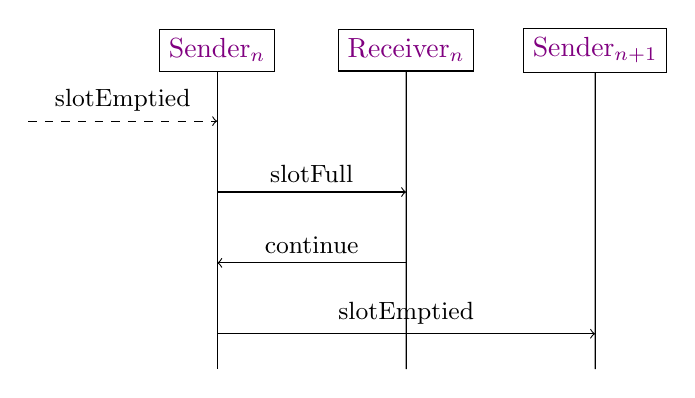
\begin{tikzpicture}[xscale = 1.2,yscale = 0.9]
\draw (0,0) node[draw](sender){ \scalacolour Sender$_n$ };
\draw (2,0) node[draw](receiver){ \scalacolour Receiver$_n$ };
\draw (4,0) node[draw](sender2){ \scalacolour Sender$_{n+1}$ };
\draw (sender) -- ++ (0,-4.5);
\draw (receiver) -- ++ (0,-4.5);
\draw (sender2) -- ++ (0,-4.5);
\draw[->,dashed] (-2,-1) -- node[above] {\small\scalastyle slotEmptied} (0,-1);
\draw[->] (0,-2) -- node[above] { \small\scalastyle slotFull} (2,-2);
\draw[<-] (0,-3) -- node[above] { \small\scalastyle continue} (2,-3);
\draw[->] (0,-4) -- node[above] {\small\scalastyle slotEmptied} (4,-4);
\end{tikzpicture}
\end{center}
\end{slide}


%%%%%


\begin{slide}
\heading{Example: a synchronous channel}

\begin{scala}
class SyncChanSemaphores[A] extends SyncChanT[A]{  
  /** The current or previous value. */
  private var value = null.asInstanceOf[A]

  /** A semaphore for signalling to receiver that a value has been deposited. */
  private val slotFull = new SignallingSemaphore

  /** A semaphore for signalling to current sender that it can continue. */
  private val continue = new SignallingSemaphore

  /** A semaphore for signalling to the next sender that the previous value has
    * been read. */
  private val slotEmptied = new MutexSemaphore
  ...
}
\end{scala}
\end{slide}

%%%%%

\begin{slide}
\heading{Example: a synchronous channel}

The three semaphores will collectively provide mutual exclusion: when any
thread is active, all semaphores will be down; when no thread is active, a
single semaphore will be up.  Initially, just |slotEmptied| is up.

There is no need to have an extra |full| variable indicating that the current
value is valid: the |slotFull| and |slotEmptied| semaphores fulfil that role. 
\end{slide}

%%%%%

\begin{slide}
\heading{Example: a synchronous channel}

\begin{scala}
  def send(x: A) = {
    slotEmptied.down       // wait for previous value to be consumed (3)
    value = x               // deposit my value
    slotFull.up             // pass baton to receiver at (1)
    continue.down           // wait for receiver (2)
    slotEmptied.up          // pass baton to next sender at (3)
  }

  def receive: A = {
    slotFull.down           // wait for sender (1)
    val result = value      // take value
    continue.up             // pass baton to current sender at (2)
    result
  }
\end{scala}
\end{slide}

%%%%%

\begin{slide}
\heading{Example: a synchronous channel}

The signals must happen in the expected order:
\[
\begin{array}{rcl@{\qquad}l}
\sm{slotEmptied.down}_1 & \prec & \sm{slotFull.up}_1 & 
  \mbox{(program order for \SCALA{send})} \\
  & \prec & \sm{slotFull.down}_1 & \sm{(signal on {\scalashape slotFull})} \\
  & \prec & \sm{continue.up}_1 & \mbox{(program order for \SCALA{receive})} \\
  & \prec & \sm{continue.down}_1 & \sm{(signal on {\scalashape continue})} \\
  & \prec & \sm{slotEmptied.up}_1 & \mbox{(program order for \SCALA{send})} \\
  & \prec & \sm{slotEmptied.down}_2 & 
     \sm{(signal on {\scalashape slotEmptied})} \\
  & \prec & \ldots
\end{array}
\]

In particular, for each semaphore $s$,\, $s.\sm{down}_n \prec
s.\sm{up}_{n+1}$, so no signal is lost.
\end{slide}

%%%%%

\begin{slide}
\heading{Example: a synchronous channel}

Here's an incorrect version, where |receive| (rather than |send|) signals on
|slotEmptied|. 
%
\begin{scala}
  def send(x: A) = {
    slotEmptied.down       // wait for previous value to be consumed (3)
    value = x               // deposit my value
    slotFull.up             // pass baton to receiver (1)
    continue.down           // wait for receiver (2)
  }

  def receive: A = {
    slotFull.down           // wait for sender (1)
    val result = value      // take value
    continue.up             // pass baton to current sender (2)
    slotEmptied.up          // pass baton to next sender at (3)
    result
  }
\end{scala}
\end{slide}

%%%%%

\begin{slide}
\heading{Example: a synchronous channel}

With the version on the previous slide, suppose a |send| is suspended just
before performing |continue.down|.  Then the current receiver can signal on
|continue| and |slotEmptied|.  Then the following sender and receiver can run,
leading to a second |continue.up|, which breaks the precondition of |up|.  If
our implementation of semaphores had allowed such a second |up|, it would have
been a lost signal.
\end{slide}

%%%%%%%%%%%%%%%%%%%%%%%%%%%%%%%%%%%%%%%%%%%%%%%%%%%%%%%

\begin{slide}
\heading{Example: first-come-first-served mutual exclusion}

Consider a mechanism to allow clients to access a shared resource
under mutual exclusion.  Suppose we also want to ensure that clients
gain access in a first-come-first-served order.  (Note that this will have a
performance overhead, but might be desirable in some circumstances.)
%
We will implement this using semaphores. 

If a process is forced to wait to access the resource, it will create a new
semaphore, place it in a queue, and then wait on it.  When a process finishes
with the resource, it will pass the baton to the process waiting on the first
semaphore in the queue (if there is one) by raising that semaphore.

We also need to record whether the resource is currently being used.  

And we need a semaphore to enforce mutual exclusion on the object's variables.
\end{slide}

%%%%%% 

\begin{slide}
\heading{Example: first-come-first-served mutual exclusion}

\begin{scala}
class MutexQueue{
  /** A queue of semaphores for waiting threads. */
  private val queue = new scala.collection.mutable.Queue[Semaphore]

  /** Is the resource busy? */
  private var busy = false

  /** Semaphore for mutual exclusion on this object's variables. */
  private val mutex = new MutexSemaphore

  // Invariant: if the mutex is up, and busy = false, then queue is empty.
  ...
}
\end{scala}
\end{slide}

%%%%%

\begin{slide}
\heading{Example: first-come-first-served mutual exclusion}

\begin{scala}
  def enter = {
    mutex.down
    if(busy){ // have to wait
      val sem = new SignallingSemaphore; queue.enqueue(sem)
      mutex.up; sem.down                  // wait turn (1)
    }
    else assert(queue.isEmpty)
    busy = true; mutex.up
  }

  def leave = {
    mutex.down; busy = false
    if(queue.nonEmpty){                 // wake up next process at (1)
      val first = queue.dequeue; first.up
    }
    else mutex.up
  }
\end{scala}
\end{slide}
 % signalling, passing the baton, queue, barrier,
                    % queue-lock
% \input{semaphores-syncchan}




%%% I don't like how this is set out.  I don't think the first version is
%%% sound.  There's a better version in
%%% /users/gavinl/Teaching/CP/Scala/ReadersWriters.

% {\advance\slideheight by 3mm
\begin{slide}
\heading{The readers and writers problem using semaphores}

We will now consider an implementation of the readers and writers problem
using semaphores. 

As before, we keep track of the number of readers and writers in the
critical section.
\begin{scala}
  /** Number of readers in the CS. */
  private var readers = 0 

  /** Number of writers in the CS. */
  private var writers = 0 
\end{scala}
\end{slide}

%%%%%

\begin{slide}
\heading{The readers and writers problem using semaphores}

We will use the technique of passing the baton.  We will have separate
semaphores for signalling (passing the baton) to readers and writers.  A
signal on these semaphores will indicate that a waiting thread can enter. 

\begin{scala}
  /** Semaphore to signal that reader can enter.
    * Indicates that writers == 0. */
  private val readerEntry = new SignallingSemaphore

  /** Semaphore to signal that writer can enter.
    * Indicates that writers == 0 && readers == 0. */
  private val writerEntry = new SignallingSemaphore
\end{scala}
\end{slide}

%%%%%

\begin{slide}
\heading{The readers and writers problem using semaphores}

We need to keep track of how many readers and writers are waiting, so an
exiting thread can know to whom to pass the baton.  We need a mutex semaphore
to protect the object variables.
%
\begin{scala}
  /** Number of readers waiting to enter. */
  private var readersWaiting = 0

  /** Number of writers waiting. */
  private var writersWaiting = 0

  /** Semaphore to protect shared variables. */
  private val mutex = new MutexSemaphore
\end{scala}
\end{slide}

%%%%%

\begin{slide}
\heading{The reader entering}

If a reader has to wait, when it is awoken, it signals to the next reader if
there is one. 
%
\begin{scala}
  def readerEnter = {
    mutex.down
    if(writers == 0){ // go straight in
      readers += 1; mutex.up
    }
    else{ // have to wait
      readersWaiting += 1; mutex.up
      readerEntry.down                         // wait to be released (1)
      assert(writers == 0); readersWaiting -= 1; readers += 1
      if(readersWaiting > 0) readerEntry.up // signal to next reader at (1)
      else mutex.up
    }
  }
\end{scala}
\end{slide}

%%%%%

\begin{slide}
\heading{The writer entering}

\begin{scala}
  def writerEnter = {
    mutex.down
    if(readers == 0 && writers == 0){ // go straight in
      writers = 1; mutex.up
    }
    else{ // have to wait
      writersWaiting += 1; mutex.up
      writerEntry.down              // wait to be released (2)
      writersWaiting -= 1
      assert(readers == 0 && writers == 0); writers = 1
      mutex.up
    }
  }
\end{scala}
\end{slide}

%%%%%

\begin{slide}
\heading{Readers and writers leaving}

A leaving reader can signal to a waiting writer.  A leaving writer can signal
to either a waiting reader or waiting writer.
%
\begin{scala}
  def readerLeave = {
    mutex.down
    readers -= 1; assert(readersWaiting == 0)
    if(readers == 0 && writersWaiting > 0)
      writerEntry.up                               // signal to writer at (2)
    else mutex.up
  }

  def writerLeave = {
    mutex.down
    writers = 0
    if(readersWaiting > 0) readerEntry.up        // signal to reader at (1)
    else if(writersWaiting > 0) writerEntry.up   // signal to writer at (2)
    else mutex.up
  }
\end{scala}
\end{slide}

%%%%%%%%%%%%%%%%%%%%%%%%%%%%%%%%%%%%%%%%%%%%%%%%%%%%%%% 

\begin{slide}
\heading{Starvation}

The previous version could cause a writer to be starved, if readers
continually enter and leave the critical section such that there is always at
least one reader.  To avoid this, we force a new reader to wait if there is
already a waiting writer.

\begin{scala}
  def readerEnter = {
    mutex.down
    if(writers == 0 && writersWaiting == 0){ // go straight in
      readers += 1; mutex.up
    }
    else{ ... } // as before
  }
\end{scala}

The assertion in |readerLeave| needs to be changed to 
\begin{scala}
  assert(readersWaiting == 0 || writersWaiting > 0)
\end{scala}
\end{slide}

%%%%%

\begin{slide}
\heading{Starvation}

On the assumption that no thread remains in the critical section for ever,
this ensures that writers collectively are not starved.  Once a writer starts
waiting, no more readers will enter the CS; eventually all readers will leave
the CS; and a writer will receive a signal.
\end{slide}

%%%%%

\begin{slide}
\heading{Fairness}

The implementation is potentially unfair to an \emph{individual} writer.  If
repeatedly several writers are waiting, a particular writer may never receive
the signal.  Likewise, a thread may never receive a signal on |mutex|
(although this is less likely). 

The implementation of a semaphore does not guarantee to be fair to each
individual waiting thread, although in practice it might be.

%% The semaphore implementation includes the option of providing fairness to each
%% thread waiting on it.
%% %
%% \begin{scala}
%%   private val mutex = MutexSemaphore(fair = true)
%%   private val readerEntry = SignallingSemaphore(fair = true)
%%   private val writerEntry = SignallingSemaphore(fair = true)
%% \end{scala}

%% ``Fair'' here means that if a thread~$t$ is waiting on semaphore~$s$, and an
%% infinite number of |up|s are performed on~$s$, then $t$ will receive one of
%% these signals.
%% %
%% Note that this is implied by the stronger property of first-in first-out.
%% %
%% Note also that there is a performance overhead associated with fairness.
\end{slide}



%%%%%%%%%%%%%%%%%%%%%%%%%%%%%%%%%%%%%%%%%%%%%%%%%%%%%%%%%%%%


%%%%%%%%%%

\begin{slide}
\heading{Counting semaphores}

The semaphores we have seen so far have been binary: they have just two
states, up and down.

A counting semaphore has a non-negative integer as its state.
%
\begin{itemize}
\item
The \SCALA{down} operation waits until the value is strictly positive, and
decrements it;

\item
The \SCALA{up} operation increments the value, waking a process if necessary.
\end{itemize}
%
The value of the semaphore can be thought of as the number of \emph{permits}
available for |down| operations. 
\end{slide}

%%%%%

\begin{slide}
\heading{Counting semaphores}

\begin{scala}
class CountingSemaphore(private var permits: Int = 0){

  def down = synchronized{
    while(permits == 0) wait()
    permits -= 1
  }

  def up = synchronized{
    permits += 1
    notify()
  }
}
\end{scala}
\end{slide}

%%%%%

\begin{slide}
\heading{A partial queue}

We can implement a queue, using a counting semaphore to block attempts to
remove elements until the buffer is non-empty.

\begin{scala}
/** A queue implemented using a counting semaphore. */
class CountingSemaphorePartialQueue[T] extends PartialQueue[T]{
  /** The queue itself. */
  private val queue = new scala.collection.mutable.Queue[T]

  /** Semaphore for mutual exclusion on queue. */
  private val mutex = new MutexSemaphore

  /** Semaphore for dequeueing.  The state of the semaphore equals
    * queue.length. */
  private val size = new CountingSemaphore(0)
  ...
}
\end{scala}
\end{slide}

%%%%%


\begin{slide}
\heading{A partial queue}

\begin{scala}
  def enqueue(v: T) = {
    mutex.down
    queue.enqueue(v)
    size.up
    mutex.up
  }

  def dequeue: T = {
    size.down
    mutex.down
    val result = queue.dequeue
    mutex.up
    result
  }
\end{scala}
\end{slide}

%%%%%



\begin{slide}
\heading{A partial queue}

Note that the order in which |dequeue| obtains the semaphores is
important.  If it were to obtain |mutex| first, and |queue| is empty,
then this would block |enqueue|, so the system would be deadlocked. 

\emph{Exercise:} adapt this example to produce a bounded buffer that cannot
hold more than $n$ pieces of data.
\end{slide}


% \begin{scala}
% class Buff[T]{
%   private val queue = new scala.collection.mutable.Queue[T];
%   private val mutex = new Semaphore; 
%   private val size = new CountingSemaphore(0);
%   ...
% }
% \end{scala}
% %
% \SCALA{queue} holds the data.  

% \SCALA{mutex} is used to ensure mutual exclusion of operations upon
% \SCALA{queue}.  

% \SCALA{size} is a counting semaphore which stores the number of elements
% currently in \SCALA{queue}; it is used to block attempts to remove elements
% when its value is~$0$.
% \end{slide}

% %%%%%

% \begin{slide}
% \heading{An unbounded buffer}

% \begin{scala}
% class Buff[T]{
%   ...

%   def add(v:T) = {
%     mutex.down;
%     queue.enqueue(v);
%     size.up; mutex.up;
%   }

%   def remove:T = {
%     size.down; mutex down;
%     val result = queue.dequeue;
%     mutex.up; return result;
%   }
% }
% \end{scala}
% \end{slide}

%%%%%

% \begin{slide}
% \heading{A bounded buffer}

% \emph{Exercise:} adapt this example to produce a bounded buffer, that cannot
% hold more than $n$ pieces of data.
% \end{slide}

%%%%%

\begin{slide}
\heading{Summary}

\begin{itemize}
\item
Semantics of semaphores;

\item
Implementing a semaphore using a monitor;

\item
Using a semaphore to enforce mutual exclusion;

\item
Dangers of deadlock;

\item
Using a semaphore for signalling;

\item
Examples;

\item
Passing the baton;

\item
Fairness;

\item
Counting semaphores.
\end{itemize}
\end{slide}

\end{document}

%%%%%%%%%%%%%%%%%%%%%%%%%%%%%%%%%%%%%%%%%%%%%%%%%%%%%%%
